\documentclass[a4paper]{article}
\usepackage{graphicx}

\setlength{\parskip}{\baselineskip}%

\begin{document}

\bibliographystyle{plain}

\title{Computer Vision in the Browser with WebGL}
\author{James Thewlis}

\maketitle

\section{Introduction}
The proposed project aims to implement a GPU-accelerated framework for Computer Vision in the web browser. Computer Vision implementations have benefited from the increased speed and parallelism of general purpose GPU technology such as Nvidia's CUDA. However, the overhead of distributing such applications has traditionally been high, requiring installation of executable files along with compatible hardware and libraries. Meanwhile, the focus of everyday computing has been shifting towards the web browser, which offers the advantage of instant delivery, but is generally considered inappropriate for real-time vision due to the inability to run compiled code unhindered. The introduction of JavaScript APIs giving access to the webcam and exposing the OpenGL ES graphics library through WebGL gives an opportunity to overcome this limitation. Although typically used for drawing 3D graphics, WebGL allows arbitrary parallel calculations to be offloaded onto the GPU through the use of Shader Programs. By these means it is hoped to create an extensible JavaScript Computer Vision framework, with an initial focus on face detection and feature tracking, giving innovative possibilities in areas such as augmented reality, web games and video chat.

\section{Background}

\subsection{Computer Vision and The Web}

The desire to integrate Computer Vision with the web has some history. Existing approaches largely make use of custom browser plugins able to run native code, such as the face detection used in Google Hangout \cite{GoogleAPI}. This has the disadvantage of requiring the user to trust and install the plugin in question, or may rely on browser-specific technology such as Microsoft's ActiveX or Google's Native Client. Adobe Flash has proved another contender \cite{flashopencv}, being a commonly installed plugin able to provide access to the webcam, but its bytecode-based VM is slower than native code, and its popularity is waning due to incompatible mobile devices and the introduction of comparable features in the HTML5 specifications.

JavaScript, the de-facto language of the web, has been applied to certain vision tasks with some success. Despite the disadvantage of being an interpreted language, recent efforts towards speeding up JavaScript engines, such as Google Chrome's V8, have led to great improvements through techniques such as JIT ("Just In Time") compilation. Another leap forward in making JavaScript suitable for Vision was the "getUserMedia" API, introduced in 2011, giving JavaScript direct access to the user's webcam (upon consent). There are existing implementations of single-image face detection in JavaScript, such as \cite{NSS} typically taking around a second to run on a 1024x768 image, and there is the more amusing cat face detector \cite{Kittydar} which takes 7 seconds. Face detection on video is also possible, but typically employs techniques such as downsizing the video or skipping frames. Upon embarking on the present project, the author could locate no similar such endeavour to implement a Vision suite in JavaScript, but fate being as it is, a similar project by the name of "jsfeat" \cite{jsfeat} appeared on the scene within a couple of weeks. The author chooses to take this as proof of current demand for vision on the web. Since jsfeat does not include GPU acceleration, it will serve as a useful baseline. In demos on its website it is able to track 100 user-specified points at 12-20 fps (640x480 resolution and depending on speed of motion) and can detect faces in real time, although it appears to be working at 160x120 effective resolution.

The effort to give JavaScript standards-based access to computational and graphical libraries that can take advantage of dedicated hardware was pioneered by the Khronos group, maintainers of the OpenGL and OpenCL specifications. These libraries are commonly used in native programs for 3D graphics and parallel computation respectively.

In 2009 Khronos began to draft a specification for WebGL, which would give JavaScript 3D drawing capabilities, through an extended context of the "canvas" element which was introduced in version 5 of the HTML specification. WebGL is based on the OpenGL ES 2.0 specification, which itself is a cut down version of OpenGL initially designed for the benefit of mobile devices, lacking OpenGL's deprecated fixed rendering pipeline (which has built in support for lighting and perspective transforms) to give a more lightweight library, leaving it to the developer to explicitly specify vertex transformations and texture values needed to render a scene. WebGL's functions and behaviour are largely identical to OpenGL ES 2.0, so resources and documentation are often applicable to both. Some additional considerations are needed for the browser-based host such as security restrictions on image access and support for web-specific data types like HTMLVideoElement for grabbing texture from a video (eg. from a webcam) on the page. The specification for WebGL 1.0 was released in 2011 and experimental support is present in the latest versions of Google Chrome and Mozilla Firefox. Safari and Opera also support WebGL although it is currently disabled by default. Microsoft's Internet Explorer does not support it, unless third party plugins are used.

Following WebGL, work was started on a WebCL specification, providing JavaScript bindings to the OpenCL parallel computation library, to allow code to be sped up using hardware on the GPU or multi-core CPU, a use case being physics calculations in games. Although it is still in draft form, implementations have been released by Nokia and Samsung in the form of browser plugins. WebCL would certainly be a strong candidate for Vision related tasks in the browser, especially given the wide use of OpenCL and Nvidia's CUDA for implementing high performance Vision systems. However, it is not yet implemented natively in any browser, and it remains to be seen whether it will be adopted by browser manufacturers. Since the goal of this project is to implement Computer Vision in current browsers with no extra steps required on behalf of the user, at the moment WebCL is unfortunately not an option, and its cousin WebGL is the only viable choice for running code on the GPU from a browser.

Despite being intended for drawing 3D graphics, OpenGL and hence WebGL is quite capable for performing arbitrary calculations, due to the use of shaders, which are programs that run on the GPU for the purpose of modifying the geometry and colour of a scene. In OpenGL there are two types of shader, vertex shaders, which specify the geometrical position in 3D given an array of vertex points and vertex-specific attributes, and fragment shaders, which specify the colour (RGB and alpha transparency) of the output pixels after rasterisation. Shaders in OpenGL are written in GLSL (The OpenGL Shader Language) a C-like language which offers many of the conveniences found in computation-oriented GPU platforms such as CUDA. An advantage of handling computation in shaders is that they operate in a parallel, computationally independent manner on many vertices or pixels, essentially the SIMD (Single Instruction Multiple Data) paradigm. This offers a large advantage over sequential computation on the CPU, provided the algorithm can be structured in such a way as to take advantage of massive parallelisation over many data elements, as is often the case with image processing algorithms where a certain operation is desired to be performed on every pixel. The fragment shader is where the main potential for parallelisation over data lies, since it can look up data in textures, run procedures, and output a value for every pixel in the canvas. However, computation in the vertex shader can also be valuable, since it precedes the fragment shader in the OpenGL pipeline and is able to pass data to it in the form of "varyings", which are vertex-specific variables then interpolated across the rasterised surface. This gives the possibility to precalculate information in the vertex shader that will be used by many pixels.

\begin{verbatim}
// Sample vertex shader for drawing in 2D
//=======================================
// Uniforms - same for all vertices
uniform vec2 uResolution;
//Attributes - vertex-specific
attribute vec2 aPosition;
attribute vec2 aTextureCoord;
// Varyings - for passing data to fragment shader
varying vec2 vTextureCoord;
void main() {
   // convert pixel coords to range -1,1
   vec2 normCoords = ((aPosition/uResolution) * 2.0) - 1.0;
   // Set the vertex at the clipspace x,y (2D) position
   gl_Position = vec4(normCoords, 0, 1);
   // pass aTextureCoord to fragment shader
   vTextureCoord = aTextureCoord;
}


// Simple fragment shader, assigns colour from texture to each pixel
//==================================================================
precision mediump float;
uniform sampler2D uSampler;

varying vec2 vTextureCoord; // from vertex shader
       
void main() {
    gl_FragColor = texture2D(uSampler, vTextureCoord);
}
\end{verbatim}

So far we have been talking about pixels and 3D vertices, which are not very useful if we want to work with 2D images or arbitrary numerical data. The trick to getting a simple 2D surface is to render a viewport-aligned rectangle (in practice, by drawing two triangles). As \cite{Greggman} describes, WebGL is essentially a 2D API if we want it to be, and we can work in pixels rather than OpenGL's "clipspace" units (which are -1.0 to 1.0) by normalising by the canvas resolution. As for passing data to the shaders, a limited amount of floating point or integer variables and arrays may be passed as "uniforms" to the shaders (which remain constant for each vertex or pixel), but for handling large data such as images and arrays textures must be used. Instead of drawing to the screen, the output may be rendered to a framebuffer with a texture attached, allowing it to be used as an input texture for another stage. Each pixel in a normal texture is 4 bytes (RGBA), which is suitable for representing some numerical data, but in many cases it is preferable to use floating points. This can be done using the WebGL extension OES\_texture\_float, which is supported on most platforms. However, until recently, there was no defined way to read back floating point values to JavaScript, requiring inventive solutions such as packing floats into bytes \cite{webgl-gpgpu}. The latest draft specifications of EXT\_color\_buffer\_half\_float \cite{colorbufhalf} and WEBGL\_color\_buffer\_float \cite{colorbuf}, amend the readPixels() function to permit float types, however it will be a matter of time before all browsers support it. In addition, when doing calculations, care should be given to the precision qualifiers offered by GLSL (highp, mediump, lowp) which alter the precision of numerical representations, at a speed/accuracy tradeoff. Per the GLSL specification, highp (normally IEEE float) may not be available in the fragment shader, and integers may be implemented as floats in the hardware, which should be taken into account when implementing algorithms.

There are various examples on the web using WebGL to improve the efficiency of calculations in simulations, such as WebGL Water \cite{Wallace} which calculates the water and caustics simulation in the shaders, 

In addition, the trick of using of OpenGL Shaders to increase performance is employed by the GPUImage library \cite{Larson} for image processing on iOS devices, and there is an implementation of the KLT tracking algorithm \cite{Sinha} on the GPU with OpenGL.

\subsection{Core Algorithms}

The seminal work on face detection is the \cite{ViolaJones01} paper, which for the first time gave reliable detection while maintaining a speed capable of real-time use. These advances were due to a combination of different techniques. Firstly, the use of the "integral image" in order to greatly reduce the number of lookups to find the sum intensity of a region in an image, requiring only four reads for an area of any size. An integral image is essentially a cumulative map of the pixel intensities (such that the value at any position tells the sum of those pixels to the top left of it), and by reading the four corners of a rectangle in an integral image, we can cancel out the area to the top and left, leaving only the sum of the area inside the rectangle. This makes it easy to compare the relative intensities of areas in images, which is fundamental to the features chosen by Viola and Jones, the Haar features (so named due to similarity with Haar Wavelets). Haar features compare the difference in brightness between regions of rectangles, in an attempt to pick up contrast variation. The feature value is the white region minus the shaded region of the rectangles in the figure. A 24x24 window is typically used for face detection, and during detection the values of Haar features at specific positions and sizes within that window (determined in the learning stage) need to be computed. 


\begin{figure}
    \centering
    
\includegraphics[width=2.0in]{integral.png}
    \caption{Integral Image. The sum of the shaded area is C-D-B+A (Wikipedia/Public Domain)}
\end{figure}

\begin{figure}
    \centering
    
\includegraphics[width=2.0in]{haar.png}
    \caption{Types of Haar Features (within larger windows) (Wikipedia/Public Domain)}
    \label{haar}
\end{figure}

Accounting for all variations in position and size (x,y,w,h) within the window there are many thousands of possible features. In order to pick a small number that are good for classifying, the method of Boosting is used (specifically AdaBoost), which allows multiple weak classifiers to be combined into one strong classifier. A weight is associated with each training sample, initially all equal, and the feature which best discriminates between the positive and negative samples is chosen. The weights are then updated such that missclassified samples using this feature are given a higher weight, and correct samples a lower one (so more effort goes towards "fixing" the missclassifications), then the feature selection is repeated with the new weights. In the end we get an ensemble of features that combined have a lower error.


\begin{figure}
    \centering
    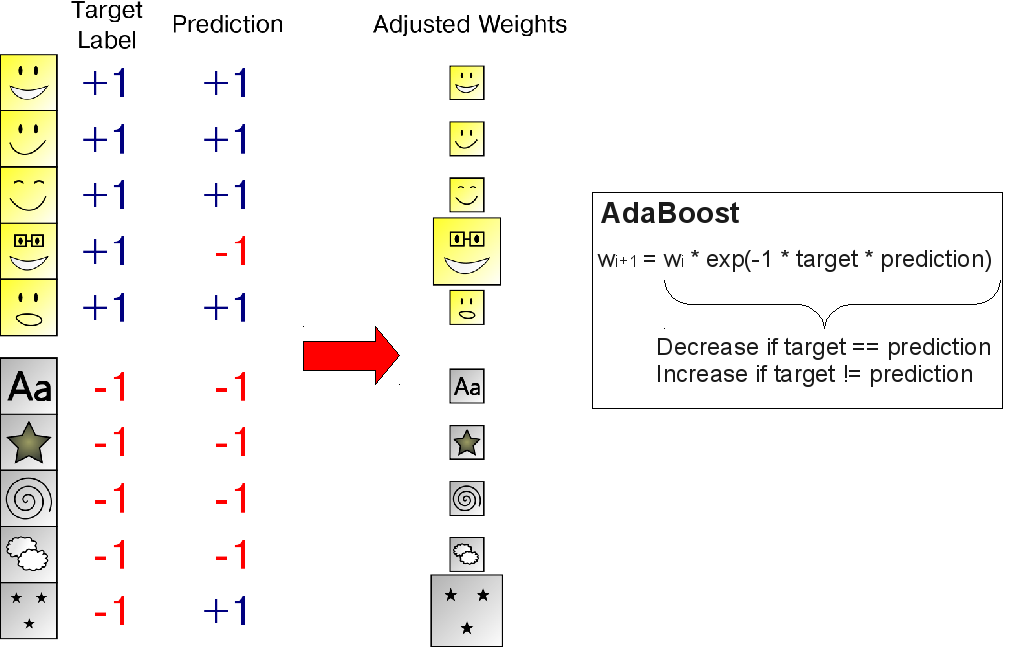
\includegraphics[width=5.0in]{adaboost.png}
    \caption{A visual illustration of Adaptive Boosting (AdaBoost), and the weight update step (Thewlis12)}
    \label{adaboost}
\end{figure}


However, with the above, during detection all the chosen features will need to be computed for all the window positions. Viola and Jones noticed that this could be improved by having a cascade of different boosted classifiers, which are decent at rejecting non-faces but will rarely reject a true face, chaining these classifiers together such that a rejected window will be immediately discarded, but an accepted window will be passed on to the next level in the cascade to face further scrutiny. This means that normally only the windows with true faces need go through every single level, whereas a non-face may be rejected right from the start. This avoids examining every single chosen feature for every single window, and makes sense intuitively since the vast majority of windows in most images will not have a face, so it is beneficial to reject them early, speeding up the procedure.

\begin{figure}
    \centering
    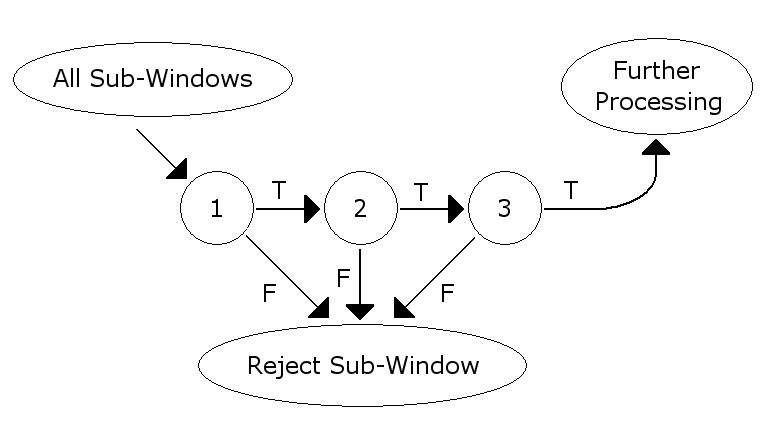
\includegraphics[width=3.0in]{cascade.png}
    \caption{The Cascade Structure (Wikipedia/Public Domain)\\ Suspected non-faces are rejected immediately, potential faces go on to further stages}
    \label{cascade}
\end{figure}

A widely used implementation of Viola Jones face detection is the OpenCV library, which provides several pre-trained cascades in an XML serialisation format. Many of the javascript face detection solutions are based on OpenCV's code.

Lienhart \cite{LienhartMaydt02} proposes an extra set of "tilted" Haar features at 45 degrees, computed thanks to a rotated integral image, in order to better represent distinctive characteristics such as slanted edges which would otherwise be missed. 

Besides Haar features, another mechanism that can be used is Local Binary Patterns (LBP). Originally used for pattern description by Ojala et al, the basic LBP simply describes the neighbourhood of a pixel in terms of whether the 8 surrounding pixels are darker or lighter than the central one, and going clockwise from the top, can be represented as an 8 bit number by writing 1 if the center is lighter, 0 otherwise.

Zhang et al extended LBP to a multi-block representation, dividing a rectangle into 3x3 blocks and comparing the outer ones with the centre, for use with face detection. Properties of LBP are that it is more robust to illumination variation, since it only records the lighter/darker relationship rather than a quantitative amount like with Haar. The ability to represent the configuration of an LBP rectangle in just one byte also makes it space efficient, especially useful when GPU textures are involved, since one could pack four patterns in one "pixel".

\begin{figure}
    \centering
    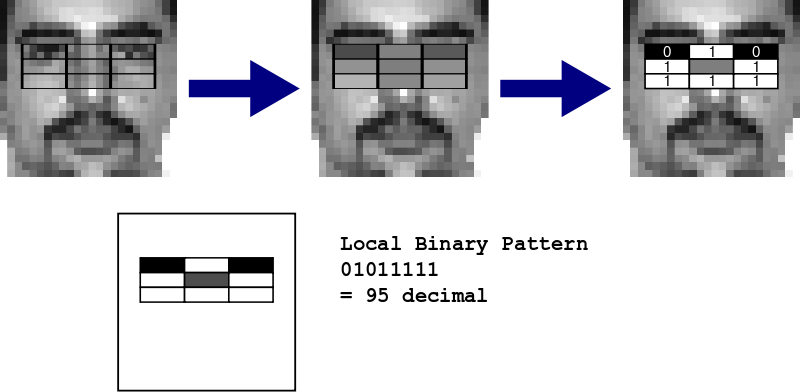
\includegraphics[width=3.0in]{lbp.png}
    \caption{Local Binary Patterns for face detection (Thewlis12)}
    \label{lbp}
\end{figure}

OpenCV also includes an LBP face detection implementation, along with a pre-trained XML file specifying a cascade for detecting frontal faces. It differs from the Haar cascades in that, for each weak classifier in a stage, rather than a simple threshold there is a list of the possible patterns (0 to 255) that contribute either positively or negatively towards a candidate window being a face, represented internally as a bit vector of size 256, made up of 8 32 bit integers.

With regards to tracking of features in an image sequence, most techniques are based in some way upon the KLT tracker. KLT, after the authors Kanade-Lucas-Tomasi, generally refers to a tracker using the results of three main papers, \cite{LucasKanade81}, \cite{TomasiKanade91} and \cite{ShiTomasi94}. The first paper deals with the problem of image registration, and proposes the method of minimising the sum of squared intensity differences in the neighbourhood of a pixel between consecutive frames. It can be used to calculate the optical flow, given small motion between the frames, by modelling the motion as a displacement of the window and recovering the displacement vector by the least squares solution to the resulting system.

The second paper expands upon this by giving a criterion for windows that are suitable for tracking, in a way that takes advantage of the registration algorithm used - "we define a feature to be good if it can be tracked well". The criterion takes into account the size of the smallest eigenvalue of the gradient matrix (structure tensor), ensuring it is above some threshold. Intuitively, two large eigenvalues represent corners and speckled patterns, and "when the smaller eigenvalue is sufficiently large to meet the noise criterion the matrix Z is usually also well conditioned". 

The third paper introduces an additional verification step to check that the features are tracked properly. This is done by taking into account affine transformations (linear warping and translation) in comparing the patch when first picked up to the patch as it is tracked. They advocate "translation for tracking because of its higher reliability and accuracy over the small interframe motion" and "affine motion for comparing features between the first and the current frame in order to monitor their quality" and propose a minimisation-style procedure to determine affine changes.

In practice, KLT implementations may use a pyramidal structure, whereby the algorithm is run on a "pyramid" of different sized versions of the frame in to compensate for the assumption the motion between frames will be small.

Since eigenvalue decomposition can be expensive, Harris corner detection \cite{HarrisStephens88} could be used instead. It is very similar to the KLT technique, but uses a measure based on the determinant and trace of the matrix to avoid computing the eigenvalue.

Existing KLT implementations include the one in the OpenCV computer vision library, the "20 years on" \cite{Baker11} Matlab project which explores various extensions, and perhaps most interestingly the GPU-based GPU\_KLT \cite{Sinha} implemented in the Cg shader language.

Further areas that would be interesting to explore include 3D facial modelling and tracking facial features in 3D, such as in \cite{Cohen00} and \cite{Caunce09}, taking advantage of the capability for 3D visualisation in WebGl. Eye tracking similar to the \cite{Opengazer} project would also be a nice feature to have, allowing gaze-based navigation or the generation of heatmaps based on where users look most.

\section{Project Plan}

\paragraph{Project Setup - done}
Read up on WebGL and JavaScript best practices, set up version control and testing suite, implement foundations for modular JavaScript library, get communication between webcam and WebGL working.

\paragraph{WebGL Interface - done}
A light wrapper around WebGL functionality, abstracting out browser-specific code and making it easier to do the things required for general purpose computation with WebGL. Various utilities for loading and passing data to shaders, and running "pipelines" of shaders by rendering to framebuffers then using the output as input to the next shader.

\paragraph{Implement Image Processing Algorithms on GPU - done}
Write shader programs to carry out various image processing algorithms, such as convolution filters, derivative images, sobel edge detection and Harris corner detection, useful for various vision algorithms such as feature tracking.

\paragraph{Face detection using Local Binary Patterns - in progress - Spring term}
\begin{itemize}
\item Support for OpenCV XML Cascade format -- parse XML vs hardcoding?
\item Implement basics of face detection in JavaScript, see where the bottlenecks are
\item Decide if integral image calculation should be done in JavaScript, on GPU (using reduction) or if there is a reliable way to get the average of a certain area by downscaling on GPU.
\item Test parallelisation strategies - over windows, over scales, over LBP rectangles?
\item Implement full GPU acceleration of feature evaluation stage
\item Test against other implementations
\item Experiment with incorporating extra information to the cascade to give hints about the locations of facial features, eg. labelling those features which are always detected in the eye area
\item And/or try other methods of singling out parts of the face
\item Write relevant sections of final report
\end{itemize}

\paragraph{Feature Tracking - in progress - Spring term}
\begin{itemize}
\item Harris corner detection for finding salient features (may change to KLT min eigenvalue)
\item Determine how to store patches, sprite-style textures?
\item Try "naive" tracking via template matching, potential fallback
\item Try KLT method to estimate displacement
\item Depending on results, try different flavours of KLT and the KLT affine quality measure
\item Test performance with different numbers of tracked features and compare with existing implementations
\item Write relevant sections of final report
\end{itemize}

\paragraph{Additional Computer Vision Algorithms - end Spring/Summer}
Depending on time, implement some more Computer Vision algorithms. Gaze tracking would be nice, but may not be very reliable with low webcam quality, would depend on quality of head tracking and ability to locate eyes, and would be hard to prevent drift from the true position. Tracking the head in 3D would be impressive and have many applications for augmented reality style things. Some sort of gesture identification or hand tracking would also be nice for manipulating things on the screen, perhaps by using stickers on fingers.

\paragraph{Create demos using framework - early Summer term}
Actually use the above algorithms to create some cool things to show off its capabilities, and demonstrate the potential for vision on the web. Both silly things like adding hats to people, and more useful like controlling perspective in a 3D world by head position, or interacting with websites in novel ways.

\paragraph{Finish writing up project - end Summer term}


\section{Evaluation Plan}

Since the main advantage offered by the GPU is speed, much of the evaluation should be centred around benchmarks and speed comparisons with other implementations. The GPU algorithms would be expected to outperform their JavaScript counterparts, such as those included in the jsfeat \cite{jsfeat} library. Comparisons with native code implementations would also be interesting, to see whether the GPU speedup is enough to overtake them despite going through JavaScript. In the case of Face Detection, the performance at different resolutions and scale sizes would show when it makes sense to use GPU acceleration, since at small sizes the overhead of transferring data to the GPU could make it lose out. Likewise for tracking, varying the number of tracked points and size of the image. Even when JavaScript-only algorithms are able to run in real time, a speed up means that you can now fit more into the update loop, allowing combinations of algorithms that would otherwise have been too slow.

However speed isn't much good when your implementation is completely broken! Although the use of the GPU will create certain constraints, which may lead to differences in behaviour, the code should be reliable and fit for its purpose. Since pre-trained face detection cascades from the OpenCV project will be used, the accuracy of detection will be determined in part by the quality of the training, but as long as it performs similarly to OpenCV with the same cascade one can be reasonably confident that the implementation is correct, and tests can be done using static images from the CMU face dataset. As for the tracking, it would probably be hard to compare two different implementations, but a qualitative assessment should show if it is working or not.

The project is novel from a technical standpoint, pushing WebGL past its original function through creative use of its support for parallel processing, but it also presents the browser with powerful new capabilities in Computer Vision, allowing for imaginative combination with all the web has to offer.


\begin{thebibliography}{9}


\bibitem[Baker11]{Baker11}
 S. Baker (2011),
 Lucas-Kanade 20 Years On,
 http://www.ri.cmu.edu/research\_project\_detail.html?project\_id=515&menu\_id=261

\bibitem[Caunce09]{Caunce09}
  A. Caunce, D. Cristinacce, C. Taylor, T. Cootes (2009),
  Locating Facial Features and Pose Estimation Using a 3D Shape Model, 
  Proc. International Symposium on Visual Computing

\bibitem[Cohen00]{Cohen00}
  M. Cohen, C. Jacobs, Z. Liu, and Z. Zhang (2000),
  Rapid Modeling of Animated Faces From Video,
  Technical Report,
  MSR-TR-2000-11

\bibitem[colorbufhalf]{colorbufhalf}
  WebGL Specification,
  WebGL EXT\_color\_buffer\_half\_float Extension Draft Specification,
  http://www.khronos.org/registry/webgl/extensions/EXT\_color\_buffer\_half\_float/

\bibitem[colorbuf]{colorbuf}
  WebGL Specification,
  WebGL\_color\_buffer\_float Extension Draft Specification,
  http://www.khronos.org/registry/webgl/extensions/WEBGL\_color\_buffer\_float/

\bibitem[flashopencv]{flashopencv}
 flashopencv
 https://github.com/bonext/flash-opencv

\bibitem[GLSL]{GLSL}
  The OpenGL ES Shading Language,
  Version 1.00 Revision 17

\bibitem[GoogleAPI]{GoogleAPI}
  Google+ API
  https://developers.google.com/+/hangouts/api/gapi.hangout.av.effects

\bibitem[Greggman]{Greggman}
  Greggman,
  WebGL Fundamentals,
  http://games.greggman.com/game/webgl-fundamentals/

\bibitem[HarrisStephens88]{HarrisStephens88}
  C. Harris and M. Stephens (1988),
  A combined corner and edge detector,
  Proceedings of the 4th Alvey Vision Conference. pp. 147–151.

\bibitem[jsfeat]{jsfeat}
jsfeat
http://inspirit.github.com/jsfeat/


\bibitem[Kittydar]{Kittydar}
  Kittydar,
  http://harthur.github.com/kittydar/


\bibitem[LienhartMaydt02]{LienhartMaydt02}
 R. Lienhart and J. Maydt (2002),
 An extended set of Haar-like features for rapid object detection,
 ICIP02, pp. I: 900–903, 2002


\bibitem[Larson]{Larson}
  B. Larson,
  GPUImage,
  https://github.com/BradLarson/GPUImage

\bibitem[LucasKanade81]{LucasKanade81}
  B. D. Lucas and T. Kanade (1981),
  An Iterative Image Registration Technique with an Application to Stereo Vision,  
  International Joint Conference on Artificial Intelligence, pages 674–679, 1981.


\bibitem[NSS]{NSS}
 A Not-so-slow JavaScript Face Detector,
 http://liuliu.me/ccv/js/nss/


\bibitem[oesfloat]{oesfloat}
  WebGL Specification,
  OES\_texture\_float Specification,
  http://www.khronos.org/registry/webgl/extensions/OES\_texture\_float/

\bibitem[Opengazer]{Opengazer}
  Opengazer,
  http://www.inference.phy.cam.ac.uk/opengazer/

\bibitem[ShiTomasi94]{ShiTomasi94}
  J. Shi and C. Tomasi (1994),
  Good Features to Track,
  IEEE Conference on Computer Vision and Pattern Recognition, pages 593–600, 1994.

\bibitem[Sinha]{Sinha}
  Sudipta Sinha,
  GPU\_KLT: A GPU-based Implementation of the Kanade-Lucas-Tomasi Feature Tracker,
  http://cs.unc.edu/\textasciitilde ssinha/Research/GPU\_KLT/

\bibitem[Thewlis12]{Thewlis12}
  J Thewlis (2012),
  Face Detection in Video for Digital Product Placement,
  Industrial Placement at MirriAd Ltd

\bibitem[TomasiKanade91]{TomasiKanade91}
  C. Tomasi and T. Kanade (1991),
  Detection and Tracking of Point Features,
  Carnegie Mellon University Technical Report CMU-CS-91-132

\bibitem[ViolaJones01]{ViolaJones01}
  P. Viola and M. Jones (2001),
  Rapid object detection using a boosted cascade of simple features,
  CVPR 2001


\bibitem[Wallace]{Wallace}
  Evan Wallace,
  WebGL Water,
  http://madebyevan.com/webgl-water/
  

\bibitem[WebglGPGPU]{webgl-gpgpu}
  WebGL GPGPU experiment - reading a floating point texture,
  http://lab.dev.concord.org/experiments/webgl-gpgpu/webgl.html





\end{thebibliography}

\end{document}

% http://www.khronos.org/registry/webgl/extensions/OES\_texture\_float/

%\begin{equation}
%    \label{simple\_equation}
%    \alpha = \sqrt{ \beta }
%\end{equation}

%\subsection{Subsection Heading Here}
%Write your subsection text here.

%\begin{figure}
%    \centering
%    \includegraphics[width=3.0in]{myfigure}
%    \caption{Simulation Results}
%    \label{simulationfigure}
%\end{figure}
